\documentclass[11pt,onecolumn]{article}
\setlength{\columnsep}{0.5cm}

\usepackage[utf8]{inputenc}
\usepackage[T1]{fontenc}
\usepackage[spanish]{babel}
\usepackage{hyperref}
\usepackage{graphicx}
\usepackage{natbib}
\usepackage{rotating}

\title{\vspace{-15mm}%
	\fontsize{24pt}{10pt}\selectfont
	\textbf{Estado del arte de la investigación sobre wikis}
	}	
\author{%
	\large
	\textsc{Emilio J. Rodríguez-Posada} \\
	\normalsize	Universidad de Cádiz \\
	\normalsize	\href{mailto:emiliojose.rodriguez@uca.es}{emiliojose.rodriguez@uca.es}
	\vspace{-5mm}
	}
\date{}


\begin{document}

\maketitle

\begin{abstract}

\end{abstract}

\section{Introducción}

%En principio lo que voy a hacer es analizar el estado del arte de la investigación de wikis, contar WikiPapers, y un poco de mi trayectoria en estos temas, cuestiones abiertas, conclusiones y trabajo futuro.

%Quizás para que fuera abordable el estado del arte, podría limitarme a clasificar los papers del último o dos últimos WikiSym. Y al último PAN/CLEF, WikiAI, MathWikis, Wikimania, WikiViz, etc. Comentar la existencia de todos estos eventos.

%Reutilizar cosas que haya escrito ya en mis papers.

%La intro la puedo adaptar del SLR que estoy haciendo de WikiPapers

El interés de los investigadores por los wikis, en especial Wikipedia, ha ido en aumento en los últimos años. La primera edición de WikiSym, un simposio sobre wikis, se celebró en 2005 y desde entonces han aparecido multitud de congresos, \emph{workshops}, conferencias y competiciones en este área. El estudio de los wikis es un campo emergente y prolífico.

Ha habido varios intentos, aunque con escaso éxito, de recopilar toda la literatura sobre wikis. Unas veces el enfoque o la herramienta utilizada eran limitados, otras debido a las dimensiones de la tarea el proyecto era abandonado y al poco tiempo los metadatos bibliográficos se perdían. En este trabajo presentamos WikiPapers, un proyecto colaborativo para recopilar toda la literatura sobre wikis. Se hace uso de MediaWiki y su extensión semántica, ambos conocidos por los investigadores de este campo. Hasta noviembre de 2012 se han recopilado más de 1.700 publicaciones y sus metadatos, además de documentación sobre herramientas y \emph{datasets} relacionados. Los metadatos son exportables en los formatos BibTeX, RDF, CSV y JSON. Los historiales completos del wiki están disponibles para descargar y facilitar su preservación. El proyecto está abierto a la participación de todo el mundo.

El resto del trabajo se divide de la siguiente manera. En la sección~2 motivamos este trabajo haciendo un repaso a los distintos enfoques utilizados hasta ahora para recopilar toda la literatura sobre wikis, incidiendo en sus ventajas e inconvenientes. En la sección~3 detallamos los objetivos. En la sección~4 definimos algunos términos que servirán para comprender mejor el contenido. En la sección~5 presentamos WikiPapers, cómo funciona y qué pasos se han dado. En la sección~6 hacemos un estado del arte empleando WikiPapers. En la sección~7 repasamos las cuestiones que a día de hoy siguen abiertas o que han tenido poca atención hasta ahora. Finalmente, en la sección~8, terminamos con unas conclusiones y trabajo futuro.

\section{Motivación}

El interés de los investigadores por los wikis, en especial Wikipedia, ha ido en aumento en los últimos años (Figura~\ref{fig:wptimeline}). La primera edición de WikiSym, un simposio sobre wikis, se celebró en 2005 y desde entonces han aparecido multitud de congresos (CLEF/PAN Lab), \emph{workshops} (WikiAI, SemWiki y MathWikis), conferencias (Wikimania, WikiCon, SMWCon, Wiki Conference India, Wikipedia Academy y Wikipedia CPOV Conference) y competiciones (WikiViz). El estudio de los wikis es un campo emergente y prolífico. Ha habido varios intentos, aunque con escaso éxito, de recopilar toda la literatura sobre wikis ~\citep{ayers2011}. Unas veces el enfoque o la herramienta utilizada eran limitados, otras debido a las dimensiones de la tarea el proyecto era abandonado y al poco tiempo los metadatos bibliográficos se perdían. Se han hecho recopilaciones en páginas personajes y blogs, a través de revisiones de literatura, haciendo uso de gestores de bibliografía, en páginas de Wikipedia y también en servicios como Zotero o CiteULike. A continuación los describimos y evaluamos sus ventajas e inconvenientes y cómo WikiPapers resuelve las carencias de estos enfoques.

\begin{figure*}[htb]
    \centering
    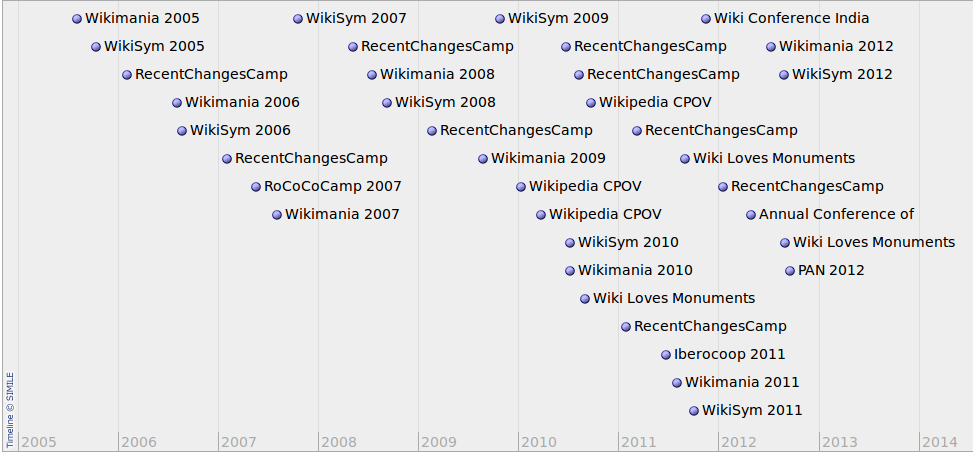
\includegraphics[width=\textwidth]{wptimeline.png} %two-column float
    \caption{Línea temporal de eventos sobre wikis.}
    \label{fig:wptimeline}
\end{figure*}

\subsection{Páginas personales y blogs}
Algunos autores han hecho recopilaciones de literatura en webs personales\footnote{\href{http://www.public.iastate.edu/~CYBERSTACKS/WikiBib.htm}{http://www.public.iastate.edu/~CYBERSTACKS/WikiBib.htm}} y blogs. Un ejemplo bastante completo de este último tipo es SWEETpedia,\footnote{\href{http://www.mkbergman.com/sweetpedia/}{http://www.mkbergman.com/sweetpedia/}} que contiene publicaciones sobre wikis y semántica. Uno de los inconvenientes de este sistema es que el esfuerzo suele recaer sobre una única persona y los metadatos no son fácilmente exportables. En WikiPapers el trabajo se hace colaborativamente y todos los metadatos son fácilmente exportables en diversos formatos.

\subsection{Gestores bibliográficos}

\subsubsection{En servidores propios}
Se han empleado gestores bibliográficos como WIKINDX\footnote{\href{http://sourceforge.net/projects/wikindx/}{http://sourceforge.net/projects/wikindx/}} creando portales propios como Wikibibliographie ENCYCLEN\footnote{\href{http://wikindx.inrp.fr/biblio_encyclen/}{http://wikindx.inrp.fr/biblio\_encyclen/}} y otros ya desaparecidos, pero como contrapartida decidieron restringir la edición a un círculo de usuarios aprobados. Sin embargo, en WikiPapers pueden participar tanto usuarios registrados como sin registrar.

%\href{http://toolserver.org/~voj/bibliography/}{http://toolserver.org/~voj/bibliography/}
%\href{http://wikiindex.org/Wiki_Research_Bibliography}{http://wikiindex.org/Wiki\_Research\_Bibliography}

\subsubsection{Servicios web y redes sociales}
Existen servicios web y redes sociales con recopilaciones de literatura sobre wikis, en Zotero,\footnote{\href{https://www.zotero.org/groups/wikipedia_research}{https://www.zotero.org/groups/wikipedia\_research}} BibSonomy\footnote{\href{http://www.bibsonomy.org/tag/wikipedia}{http://www.bibsonomy.org/tag/wikipedia}} \footnote{\href{http://www.bibsonomy.org/tag/wiki}{http://www.bibsonomy.org/tag/wiki}} y CiteULike.\footnote{\href{http://www.citeulike.org/tag/wikipedia}{http://www.citeulike.org/tag/wikipedia}}\footnote{\href{http://www.citeulike.org/tag/wiki}{http://www.citeulike.org/tag/wiki}}\footnote{\href{http://www.citeulike.org/group/382}{http://www.citeulike.org/group/382}} Este enfoque sí hace uso de una comunidad de usuarios para procesar las publicaciones, pero de nuevo requieren registrarse, y la capacidad de estos servicios para aprovechar los metadatos generando tablas o gráficos es inexistente.

\subsection{Recopilaciones en Wikipedia}
También existen listados de publicaciones y recursos en algunas Wikipedias, como en la versión alemana\footnote{\href{http://de.wikipedia.org/wiki/Wikipedia:Wikipedistik/Bibliographie}{http://de.wikipedia.org/wiki/Wikipedia:Wikipedistik\\ /Bibliographie}} y la inglesa\footnote{\href{http://en.wikipedia.org/wiki/Wikipedia:Academic_studies_of_Wikipedia}{http://en.wikipedia.org/wiki/Wikipedia:Academic\\ \_studies\_of\_Wikipedia}}. El principal inconveniente de este enfoque es que no es posible jugar con los datos dentro del mismo wiki, al estar todo escrito como texto plano, sin enriquecimiento semántico. En WikiPapers todos los metadatos son propiedades semánticas, tanto en las llamadas \emph{infoboxes} (tablas) como en el cuerpo del artículo.

\subsection{Revisiones de literatura}
Finalmente, se han realizado varias revisiones de literatura con diferente grado de exhaustividad. La primera de ellas ~\citep{voss2005} se hizo en un momento en el que las publicaciones eran escasas, pero ya se podía ver una tendencia de publicación creciente y la presencia de muchas preguntas por responder. Un año más tarde ~\citep{ayers2006} vuelve a hacer un repaso a la literatura existente y enumera aquellas áreas que han recibido interés: historiales, páginas de discusión, contenido de los artículos, políticas del sitio, citas a artículos, encuestas a usuarios y listas de correo.

No sería hasta 3 años después cuando \cite{okoli2009b} presentan una propuesta de protocolo para hacer un mapeo sistemático de la literatura sobre Wikipedia, indicando la existencia de más de 1.000 publicaciones y ese mismo año \cite{okoli2009} analiza el estado del arte. Dos años más tarde, \cite{nielsen2011} hace la mayor revisión de literatura en un documento de más de 50 páginas, en progreso e inacabado, que incluye 300 referencias a publicaciones y reincide en la existencia de 1.000 publicaciones sobre el tema.

\cite{martin2011} hace primero un repaso técnico a la estructura de la base de datos (páginas, usuarios, texto), luego se centra en las áreas de calidad y acaba con unas consideraciones filosóficas.

\cite{okoli2012} hacen una revisión de la literatura y han creado un wiki reutilizando las plantillas, formularios, semántica y estructura de WikiPapers. Están trabajando en el análisis de un subconjunto de la literatura, en este caso la relativa a Wikipedia exclusivamente. Es un proyecto temporal y pretenden incorporar sus resultados a WikiPapers.

La revisión más reciente \cite{jullien2012} hace un repaso por las motivaciones para contribuir, roles, estructura, la vida de un artículo, calidad, experiencia de usuario y accesibilidad, entre otros.

Uno de los inconvenientes de estas revisiones de literatura es que quedan rápidamente desactualizadas debido al ritmo con el que aparecen nuevas publicaciones. WikiPapers es actualizado continuamente por su comunidad de voluntarios.

\section{Objetivos}

Los objetivos de este proyecto de investigación son:

\begin{enumerate}
\item Idear un sistema o adaptar alguno existente que permita recopilar literatura sobre wikis, superando las carencias de los enfoques usados anteriormente
\item Deberá permitir añadir, eliminar y modificar metadatos bibliográficos fácilmente, de manera manual y por lotes importando contenido
\item Usará características de la web semántica para poder sacar el máximo provecho posible a los metadatos, relacionando conceptos, agrupando elementos comunes, etc
\item Tendrá licencia libre (por tanto los contenidos serán reutilizables por terceros) y facilitará exportación de los metadatos
\item Realizar un estado del arte haciendo uso del sistema creado en los puntos anteriores
\end{enumerate}

\section{Definiciones, acrónimos y abreviaturas}

%Mirar las que definí en mi PFC y meter otras más nuevas

A continuación se incluyen algunas \textbf{definiciones, acrónimos y abreviaturas} que facilitan la comprensión de este trabajo.

\textbf{Administrador}: Persona que se dedica al mantenimiento de un sistema o red. En Wikipedia hace referencia a aquellos usuarios que pueden borrar/restaurar páginas, bloquear/desbloquear usuarios y proteger/desproteger páginas.

\textbf{Anónimo}: Usuario que no se ha registrado en el wiki y aparece identificado por su dirección IP.

\textbf{API}: Application Programming Interface. La API de MediaWiki propociona acceso a los contenidos de las bases de datos.

\textbf{Artículo}: Página de un wiki situada en el espacio de nombres 0.

\textbf{Blanqueo}: Eliminación parcial o total del contenido de una página, lo que constituye una edición maliciosa o un acto de vandalismo.

\textbf{Bloqueo}: Suspensión temporal o indefinida a un usuario de su capacidad de modificar páginas. Los bloqueos sólo pueden realizarlos los administradores.

\textbf{Bot}: Programa que realiza tareas aburridas y tediosas de manera automática.

\textbf{Cambios recientes}: Página especial de los wikis en la que puede observarse las modificaciones realizadas.

\textbf{Cultura libre}: La componen todas las obras que tienen una licencia libre.

\textbf{Dataset}: Conjunto de datos con una estructura determinada que facilita su procesamiento.

\textbf{Diff}: Extracto que muestra las diferencias de contenido entre dos versiones distintas de una misma página.

\textbf{Discusión}: Anexo a cualquier página del software MediaWiki en la que se pueden discutir cambios en el contenido de dicha página.

\textbf{Edición}: Modificación de una página del wiki.

\textbf{Espacio de nombres}: División que realiza el software MediaWiki para diferenciar distintos tipos de páginas. Los principales son: artículos, categorías, plantillas y páginas de usuario.

\textbf{Etiqueta}: También conocida como netiquette, son una serie de normas de convivencia en comunidades en línea.

\textbf{Expresión regular}: Patrón que describe una o varias cadenas.

\textbf{Fork}: Bifurcación de un proyecto en dos distintos.

\textbf{GLAM}: acrónimo de Galerías, Bibliotecas, Archivos y Museos.

\textbf{Historial}: Conjunto formado por todas las versiones anteriores de una misma página, incluida la actual. Cada página mantiene su propio historial y es utilizado frecuentemente para restaurar el contenido debido a vandalismos, desacuerdos en la redacción, etc.

\textbf{Interwiki}: Vínculo que une a dos páginas sobre un mismo tema en distintos idiomas.

\textbf{Los cinco pilares}: Las cinco normas básicas de Wikipedia y en las que se sustentan el resto de políticas: (1) Wikipedia es una enciclopedia, (2) Wikipedia busca el punto de vista neutral, (3) Wikipedia es de contenido libre, (4) Wikipedia sigue unas normas de etiqueta, (5) Wikipedia no tiene normas firmes más allá de estos cinco pilares.

\textbf{Motor wiki}: software que facilita la redacción de documentos de manera colaborativa a través de una red.

\textbf{Namespace}: véase \textbf{Espacio de nombres}.

\textbf{NPOV}: véase \textbf{Punto de vista neutral}.

\textbf{Política}: Norma refrendada por la comunidad. Aunque Wikipedia no tiene normas firmes más allá de los cinco pilares, se recomienda seguir las políticas del proyecto, pues han sido elaboradas con un alto consenso y su no cumplimiento puede acarrear sanciones como bloqueos.

\textbf{Preservación digital}: tareas que permiten conservar datos digitales largo tiempo.

\textbf{Punto de vista neutral}: Es uno de los pilares de Wikipedia. Según el texto de la política oficial de Wikipedia en español: «El punto de vista neutral (PVN) establece que la enciclopedia debe contener hechos y que sus artículos deben ser escritos sin sesgos, presentando adecuadamente todos los puntos de vista existentes sobre tales hechos. [...] Esta política se malinterpreta con facilidad. No supone que sea posible escribir un artículo desde un único punto de vista objetivo no sesgado. Dice que debemos representar adecuadamente los diferentes puntos de vista y sin que el artículo afirme, implique o insinúe que alguno de ellos es el correcto. La neutralidad es mostrar todos los puntos de vista relevantes posibles tal y como son, para que cada lector adopte la opinión que prefiera».

\textbf{Regexp}: véase \textbf{Expresión regular}.

\textbf{Resumen de edición}: Texto que puede adjuntarse a cada modificación de una página con el propósito de explicar en qué consisten los cambios realizados. Es útil cuando se consulta el historial. Se considera una buena práctica el rellenarlo.

\textbf{Reversión}: Restaurar el contenido de una página a su estado anterior.

\textbf{Semántica}: 

\textbf{Spam}: mensaje publicitario no deseado.

\textbf{Usabilidad}: define la facilidad de uso de una aplicación.

\textbf{Vandalismo}: Modificación no deseada y maliciosa en la que se elimina parte de la información, se introducen palabras soeces, etc.

\textbf{Web 2.0}: Término acuñado por Tim O'Reilly y que hace referencia a una nueva generación de la web, caracterizada por una mayor participación de los usuarios en los contenidos.

\textbf{Wiki}: Sitio web que permite a sus visitantes modificar el contenido del mismo. Ward Cunningham, desarrollador del primer software wiki, llamado WikiWikiWeb, lo definió como «the simplest online database that could possibly work».

\textbf{Wikifarm}: sitio que ofrece hosting para wikis.


\section{WikiPapers}

%descripción del proyecto

WikiPapers\footnote{\href{http://wikipapers.referata.com}{http://wikipapers.referata.com}} fue lanzado en abril de 2011 (Figura~\ref{fig:wpfull}). Haciendo uso de MediaWiki y su extensión semántica, recopila de manera colaborativa información acerca de toda la literatura sobre wikis, así como de herramientas y \emph{datasets} relacionados. No hace falta estar registrado para participar, aunque es recomendable.

WikiPapers agrupa todas las ventajas de los sistemas mencionados anteriormente y soluciona sus inconvenientes. Permite hacer listados específicos de publicaciones, similares a SWEETpedia: por poner un ejemplo, existe uno de revisiones de literatura.\footnote{\href{http://wikipapers.referata.com/wiki/List_of_literature_reviews}{http://wikipapers.referata.com/wiki/List\_of\\ \_literature\_reviews}} Funciona como un gestor bibliográfico, al almacenar los metadatos de las publicaciones y permitir hacer búsquedas, filtrarlos o exportarlos, individualmente o en conjunto. También facilita que grupos de usuarios se comuniquen a través de las páginas de discusión y compartan información sobre publicaciones de su interés, funcionando como una red social. Por otro lado, el espacio de discusión debajo de cada página posibilita a los lectores hacer valoraciones de los artículos. Y al ser un wiki, puede ser constantemente mejorado, evitando quedar desactualizado debido al rápido ritmo de publicación.

Desde un punto de vista más estadístico, es posible generar gráficas y tablas a partir de los metadatos disponibles en WikiPapers, aprovechando así la capacidad que ofrece la semántica. Gráficos de barras, circulares o líneas temporales están presentes y facilitan la visualización y comprensión de la información. También existe la posibilidad de incrustar diapositivas (SlideShare) y vídeos (YouTube, Vimeo).

Finalmente, el wiki y sus historiales están disponibles tanto para su descarga en XML y accesible a través de la API de MediaWiki. Esto impide que todo el trabajo se pierda, como ha sucedido en otros proyectos que quedaron inactivos y finalmente desaparecieron.

\begin{figure}[htb]
\centering
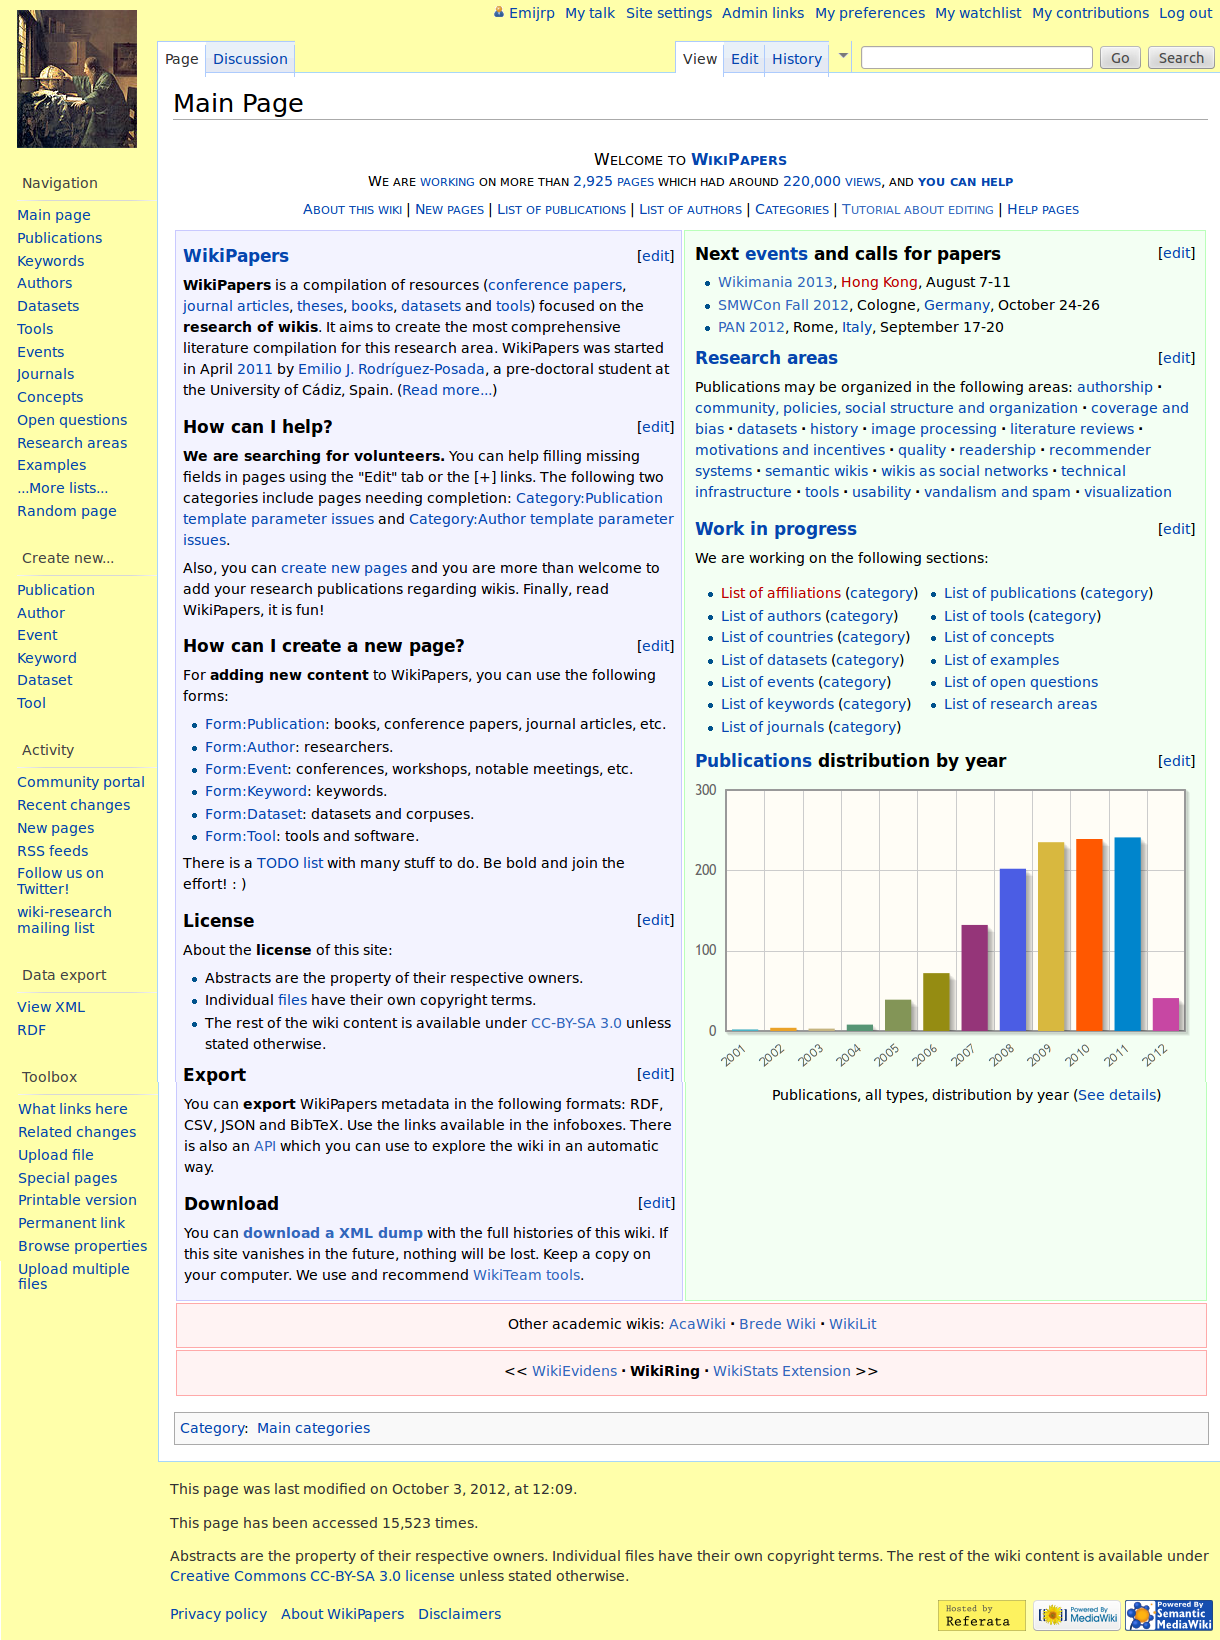
\includegraphics[width=0.9\textwidth]{wpfull.png}
\caption{Portada de WikiPapers.}
\label{fig:wpfull}
\end{figure}

\subsection{Publicaciones}
En WikiPapers cada publicación dispone de una página en la que se detallan todos sus metadatos (título, autores, palabras clave, año, revista o congreso, DOI, idioma, licencia, enlaces al fichero y motores de búsqueda), el abstract, las referencias que incluye, las citas que recibe y un espacio de discusión. Los metadatos sirven para hacer búsquedas y filtrar. A noviembre de 2012 ya se dispone de más de 1.700 publicaciones,\footnote{\href{http://wikipapers.referata.com/wiki/List_of_publications}{http://wikipapers.referata.com/wiki/List\_of\_publications}} incluyendo artículos de revistas y congresos, tesis y libros. Todos los metadatos se pueden exportar en los formatos BibTeX, RDF, CSV y JSON.

\subsection{Palabras clave}
Existe un listado de todas las palabras clave\footnote{\href{http://wikipapers.referata.com/wiki/List_of_keywords}{http://wikipapers.referata.com/wiki/List\_of\_keywords}} presentes en los artículos y cada una de ellas cuenta con varios términos relacionados, lo que permite navegar entre ellas. Las más frecuentes son: Wikipedia, wiki, semantic wiki, web 2.0, collaboration, evaluation, collaborative learning, knowledge management, MediaWiki, motivation, data mining y conflict. 

\subsection{Autores}
Para cada autor hay una ficha que incluye su nombre, afiliación, país, índice de coautores, página web, estadísticas sobre número de publicaciones y citas, y por supuesto un listado de publicaciones, \emph{datasets} y herramientas de su creación. Ya están listados unos 1.000 autores.\footnote{\href{http://wikipapers.referata.com/wiki/List_of_authors}{http://wikipapers.referata.com/wiki/List\_of\_authors}}

\subsection{Datasets}
Un listado de \emph{datasets}\footnote{\href{http://wikipapers.referata.com/wiki/List_of_datasets}{http://wikipapers.referata.com/wiki/List\_of\_datasets}} permite observar la gran cantidad de datos sobre comunidades wiki disponibles para analizar. Existen \emph{datasets} sobre vandalismo, texto wiki enriquecido con semántica, datos extraidos de \emph{infoboxes}, \emph{logs} anonimizados de visitas, mensajes de listas de correo y por supuesto los historiales de Wikipedia.

A este respecto, el proyecto WikiTeam\footnote{\href{http://code.google.com/p/wikiteam/}{http://code.google.com/p/wikiteam/}} está compilando una gran cantidad de datos sobre comunidades wiki, que se cifra ya en 4.500 \emph{dumps}.

\subsection{Herramientas}
Se está construyendo un listado de herramientas\footnote{\href{http://wikipapers.referata.com/wiki/List_of_tools}{http://wikipapers.referata.com/wiki/List\_of\_tools}} que se han desarrollado a la hora de investigar sobre wikis y para proponer soluciones a ciertos problemas.

\subsection{Y más...}
También se está recopilando información sobre revistas, congresos, eventos, conceptos, ejemplos de análisis, preguntas abiertas, encuestas, motores wiki, wikifarms y más. WikiPapers, además de todo lo comentado anteriormente, sirve para que investigadores de wikis hagan comunidad y establezcan conexiones para futuras investigaciones.


\section{Estado del arte}

%Áreas de investigación \href{http://wikipapers.referata.com/wiki/List_of_research_areas}{http://wikipapers.referata.com/wiki/List\_of\_research\_areas}

A continuación se realiza un repaso de la literatura, dividiendo el estudio de los wikis en una serie de parcelas bien definidas.

\subsection{Autoría y calidad}

WikiTrust, comparación Nature


\subsection{Cobertura y sesgos}


\subsection{Comunidad}


\subsection{Educación}

Wikis como herramientas educativas

Experiencias docentes


\subsection{Datasets}

Una de las ventajas de la investigación sobre wikis, sobre todo el caso de Wikipedia, es la disponibilidad de \emph{datasets} con los textos completos, historiales, \emph{logs} e información de actividad de los usuarios.

La mayoría de los wikis cuenta con algún tipo de licencia libre, generalmente Creative Commons o GFDL, lo que facilita la adquisición, uso y distribución de los datos, aunque son pocos los que ponen a disposición del público copias completas de las bases de datos. Esto está cambiando a raiz de la aparición de WikiTeam, un proyecto para desarrollar herramientas para preservar wikis, que fundé en 2011 y que ya ha generado datasets para más de 5000 wikis.

Otros datasets sobre wikis que están disponibles se encuentran en la tabla \ref{tab:datasetstable}. Incluyen datos sobre coordenadas de artículos, semántica, páginas borradas, red de enlaces entre páginas, vandalismo, enlaces externos a repositorios, taxonomías y otros.

\href{http://wikipapers.referata.com/wiki/List_of_datasets}{http://wikipapers.referata.com/wiki/List\_of\_datasets}

\begin{sidewaystable}[h]
\centering
\begin{tabular}{| c | c | c | c |}
\hline
\textbf{Dataset} & \textbf{Tamaño} & \textbf{Idioma} & \textbf{Descripción} \\
\hline
CoCoBi & · & Alemán & · \\ \hline 
Coordinates in Wikipedia articles & · & Multilingüe & · \\ \hline 
DBpedia & · & Multilingüe & · \\ \hline 
DeletionPedia & · & Inglés & · \\ \hline 
Domas visits logs & · & Multilingüe & · \\ \hline 
Google dataset linking strings and concepts & · & Multilingüe & · \\ \hline 
PAN Wikipedia vandalism corpus 2010 & · & Inglés & · \\ \hline 
PAN Wikipedia vandalism corpus 2011 & · & Multilingüe & · \\ \hline 
PlusPedia & · & Alemán & · \\ \hline 
Repos-2012-dataset & · & Multilingüe & · \\ \hline 
Social networks of Wikipedia dataset & · & · & · \\ \hline 
WikiBiography & · & · & · \\ \hline 
WikiCorpus & · & Multilingüe & · \\ \hline 
WikiIndex & · & Inglés & · \\ \hline 
WikiNet & · & Multilingüe & · \\ \hline 
WikiPapers & · & Inglés & · \\ \hline 
WikiRelations & · & Inglés & · \\ \hline 
WikiTaxonomy & · & · & · \\ \hline 
WikiTeam dumps & · & Multilingüe & · \\ \hline 
Wikia dumps & · & Multilingüe & · \\ \hline 
Wikimedia dumps & · & Multilingüe & · \\ \hline 
Wikipedia Historical Attributes Data & · & Inglés & · \\ \hline 
Wikipedia Vandalism Corpus (West) & · & Inglés & · \\ \hline 
Wikipedia page-to-page link database & · & Inglés & · \\ \hline 
WikipediaXML & · & Multilingüe & · \\ \hline 
Wlm-2011-dataset & · & Multilingüe & · \\ \hline
\end{tabular}
\caption{Datasets relacionados con wikis.}
\label{tab:datasetstable}
\end{sidewaystable}

\subsection{GLAM}


\subsection{Herramientas}

Entorno a los wikis se generado un espectro de herramientas específicas. Unas (Figura~\ref{tab:vandaltoolstable}) ayudan a detectar, reparar y eliminar vandalismos y ataques de spam, uno de los pocos inconvenientes que tienen los wikis al ser sistemas tan abiertos a la colaboración. Otras herramientas, más enfocadas a la investigación, facilitan el acceso a los datos de los wikis (Figura~\ref{tab:frameworkstable}), a procesarlos (Figura~\ref{tab:dataprocessingtoolstable}) y visualizarlos (Figura~\ref{tab:visualizationtoolstable}).

\href{http://wikipapers.referata.com/wiki/List_of_tools}{http://wikipapers.referata.com/wiki/List\_of\_tools}

\begin{sidewaystable}[h]
\centering
\begin{tabular}{| c | c | c | c | c |}
\hline
\textbf{Herramienta} & \textbf{S.O.} & \textbf{Idioma} & \textbf{Licencia} & \textbf{Descripción} \\
\hline
AVBOT & Multiplataforma & Español & GPL & Bot anti-vandalismo para Wikipedia en español. \\ \hline
ClueBot & GNU/Linux & · & · & · \\ \hline
CryptoDerk's Vandal Fighter & Multiplataforma & Inglés & · & · \\ \hline
Huggle & Windows & · & GPL & · \\ \hline
Igloo & · & · & · & · \\ \hline
STiki & Multiplataforma & Inglés & GPL & · \\ \hline
Salebot & · & · & · & · \\ \hline
Twinkle & · & · & · & · \\ \hline
Vandal Fighter & Multiplataforma & Inglés & · & · \\ \hline
VandalProof & Windows & Inglés & · & · \\ \hline
VandalSniper & Multiplataforma & Inglés & · & · \\ \hline
\end{tabular}
\caption{Herramientas anti-vandalismo y anti-spam.}
\label{tab:vandaltoolstable}
\end{sidewaystable}


\begin{sidewaystable}[h]
\centering
\begin{tabular}{| c | c | c | c | c |}
\hline
\textbf{Herramienta} & \textbf{S.O.} & \textbf{Idioma} & \textbf{Licencia} & \textbf{Descripción} \\
\hline
Java Wikipedia Library & Multiplataforma & Inglés & LGPL & Framework en Java. \\ \hline
Perlwikipedia & Multiplataforma & Inglés & GPL & Framework en Perl. \\ \hline
Python-wikitools & Multiplataforma & Inglés & GPL & Framework en Python. \\ \hline
Pywikipediabot & Multiplataforma & Inglés & MIT license & Frame work en Python. El más usado. \\ \hline
\end{tabular}
\caption{Frameworks.}
\label{tab:frameworkstable}
\end{sidewaystable}


\begin{sidewaystable}[h]
\centering
\begin{tabular}{| c | c | c | c | c |}
\hline
\textbf{Herramienta} & \textbf{S.O.} & \textbf{Idioma} & \textbf{Licencia} & \textbf{Descripción} \\
\hline
JWordNet-Similarity & Multiplataforma & Inglés & · & · \\ \hline 
Manypedia.com & Multiplataforma & Inglés & Affero GPL & · \\ \hline 
Wikokit & Multiplataforma & Inglés & Varias & · \\ \hline 
Zawilinski & Multiplataforma & · & · & · \\ \hline 
\end{tabular}
\caption{Herramientas sobre el lenguaje.}
\label{tab:languagetoolstable}
\end{sidewaystable}


\begin{sidewaystable}[h]
\centering
\begin{tabular}{| c | c | c | c | c |}
\hline
\textbf{Herramienta} & \textbf{S.O.} & \textbf{Idioma} & \textbf{Licencia} & \textbf{Descripción} \\
\hline
DiffDB & · & · & · & · \\ \hline 
Ikiwiki & · & · & · & · \\ \hline 
Infobox2rdf & · & · & · & · \\ \hline 
MediaWiki API & · & · & · & · \\ \hline 
Sioc MediaWiki & · & · & · & · \\ \hline 
Wiki Edit History Analyzer & · & · & · & · \\ \hline 
Wiki2XML parser & · & · & · & · \\ \hline 
WikiPrep & · & · & · & · \\ \hline 
Wikihadoop & · & · & · & · \\ \hline 
Wikimedia Utilities & · & · & · & · \\ \hline 
Wikipedia Extractor & · & · & · & · \\ \hline 
Wikipedia Miner & · & · & · & · \\ \hline 
Wikipedia-map-reduce & · & · & · & · \\ \hline 
\end{tabular}
\caption{Herramientas de procesamiento de datos.}
\label{tab:dataprocessingtoolstable}
\end{sidewaystable}


\begin{sidewaystable}[h]
\centering
\begin{tabular}{| c | c | c | c | c |}
\hline
\textbf{Herramienta} & \textbf{S.O.} & \textbf{Idioma} & \textbf{Licencia} & \textbf{Descripción} \\
\hline
HistoryFlow & · & · & · & · \\ \hline 
StatMediaWiki & · & · & · & · \\ \hline 
Wiki Explorator & · & · & · & · \\ \hline 
Wiki Trip & · & · & · & · \\ \hline 
WikiBlame & · & · & · & · \\ \hline 
WikiChanges & · & · & · & · \\ \hline 
WikiEvidens & · & · & · & · \\ \hline 
WikiPride & · & · & · & · \\ \hline 
WikiScanner & · & · & · & · \\ \hline 
WikiTracer & · & · & · & · \\ \hline 
WikiTrust & · & · & · & · \\ \hline 
WikiVis (FH-KL) & · & · & · & · \\ \hline 
WikiVis (UM) & · & · & · & · \\ \hline 
WikiWarMonitor & · & · & · & · \\ \hline 
WikiXRay & · & · & · & · \\ \hline 
Wikistream & · & · & · & · \\ \hline 
Wmcharts & · & · & · & · \\ \hline 
\end{tabular}
\caption{Herramientas de visualización.}
\label{tab:visualizationtoolstable}
\end{sidewaystable}


\begin{sidewaystable}[h]
\centering
\begin{tabular}{| c | c | c | c | c |}
\hline
\textbf{Herramienta} & \textbf{S.O.} & \textbf{Idioma} & \textbf{Licencia} & \textbf{Descripción} \\
\hline
WikiSim & · & · & · & · \\ \hline 
WikiTeam tools & · & · & · & · \\ \hline 
· & · & · & · & · \\ \hline 
\end{tabular}
\caption{Otras herramientas.}
\label{tab:othertoolstable}
\end{sidewaystable}



\subsection{Historiales}


\subsection{Infraestructura}

por ejemplo los wikis al estilo p2p para repartir la carga... había una tesis sobre eso en danés?


\subsection{Motivaciones e incentivos}


Encuestas...

\subsection{Motores wiki}

Aunque MediaWiki sea el motor wiki más conocido y utilizado, hay muchos otros. Existe un portal que enumera a la mayoría de ellos, llamado WikiMatrix\footnote{\href{http://www.wikimatrix.org}{http://www.wikimatrix.org}}. Contiene información acerca de más de 125 motores wiki y permite hacer comparaciones sobre la presencia o carencia de funcionalidades. La existencia de tantos motores dificulta la interoperabilidad entre ellos y existen intentos de unificar o al menos promover una sintaxis estándar, como el proyecto WikiCreole\footnote{\href{http://www.wikicreole.org}{http://www.wikicreole.org}}.

\subsection{Preservación}

urobe, revisar el paper de wikiteam

\subsection{Procesamiento de imágenes}

Poquísimo hay hecho me parece a mí...

\subsection{Procesamiento del Lenguaje Natural}


\subsection{Recomendación de tareas}

Images for bio

\subsection{Semántica}

SWEETpedia

\subsection{Usabilidad}


\subsection{Vandalismo y spam}

Bots y algoritmos, flaggedrevs, abusefilter, extensiones anti-spam

 \citep{avbot2011}
 \citep{avbot2010}
 \citep{avbot2009}

\subsection{Visualización}

WikiViz y todas las herramientas de visualización...


\subsection{Wikifarms}

 \citep{kittur2010}

\subsection{Wikis como redes sociales}


\section{Cuestiones abiertas}



\section{Conclusiones y trabajo futuro}
porqué hacía falta WikiPapers
aglutina todas las ventajas de los anteriores sistemas
lo que se ha hecho, cifras,
lo que queda por hacer y como ayudar
el futuro y más allá...



\bibliographystyle{wink}        
\bibliography{proyecto-investigacion-2012}

\section*{Licencia}
Esta obra está bajo licencia \href{http://creativecommons.org/licenses/by-sa/3.0/}{Creative Commons Reconocimiento-CompartirIgual 3.0 Unported}.

\end{document}
